\chapter{OTFVis Visualizer}
\label{ch:otfvis}
% ##################################################################################################################

\hfill \textbf{Authors:} Kai Nagel, Michael Zilske ???

\begin{center} 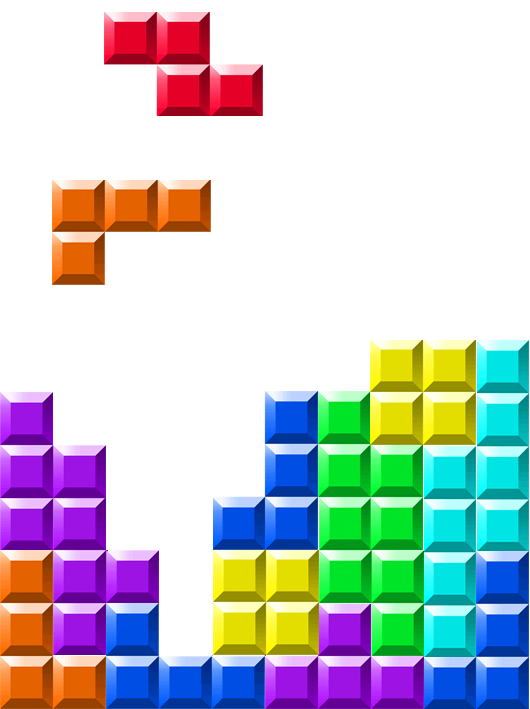
\includegraphics[width=0.25\textwidth, angle=0]{figures/MATSimBook.png} \end{center}

% ##################################################################################################################
\begin{compactitem}
\item Invoking the module: run \lstinline|org.matsim.contrib.otfvis.OTFVis|
\item Configuration: \lstinline|otfvis| configuration file section
\item Code: \lstinline|org.matsim.contrib.otfvis|
\end{compactitem}

Before senozon via the OTFVis (on-the-fly visualizer) \citep[][]{Strippgen_PhDThesis_2009} was the main visualization tool of MATSim. OTFVis is able to visualize results during runtime of a MATSim run. It is available as a contribution. It is implemented in java, however, to make use of sophisticated visualization of the OpenGL framework, it is also heavily based on jogl. This requires a couple of user actions to get jogl running on his specific platform. 

%This platform dependency has lead to some issue with the programs stability. It is thus recommended to use the senozon via. visualizer.
%\michaz{The jogl and stability issues aren't true anymore, it runs out of the box everywhere and hasn't broken for quite some time. I also recommend using via, but only because otfvis is otfvis, not because of jogl. :-)}

% ################################################################################################################





